%% ========================================================================
%% chapter4.tex -- Chapter 4: Solution / Design and Implementation
%% Topic: Current-stage benchmark implementation for SAM-family polyp segmentation
%% Last updated: 2026-06-25
%% ========================================================================

\chapter{Solution: Design and Implementation}
\label{chap:solution}

This chapter follows the ``Solution (or Design and Implementation)'' role in the BNBU partial-thesis template. Chapter~\ref{chap:outline} defined the research methodology at the protocol level: datasets, prompts, metrics, baseline taxonomy, and caveats. This chapter explains how that methodology is applied as a reproducible benchmark system. The chapter therefore focuses on implementation design rather than on quantitative interpretation; the numerical validation of the system is reported in Chapter~\ref{chap:validation}.

The central design principle is to separate \emph{method-specific model execution} from the \emph{shared evaluation contract}. Each baseline keeps its own loading and inference path, because SAM, MedSAM, SAM2, PP-SAM, SAMed, ASPS, and OP-SAM expose different model interfaces. At the same time, the evaluation split, prompt rule, metric definitions, and artifact schema are kept as consistent as possible. This separation allows the project to compare methods without hiding protocol differences inside the implementation.

\begin{figure}[H]
\centering
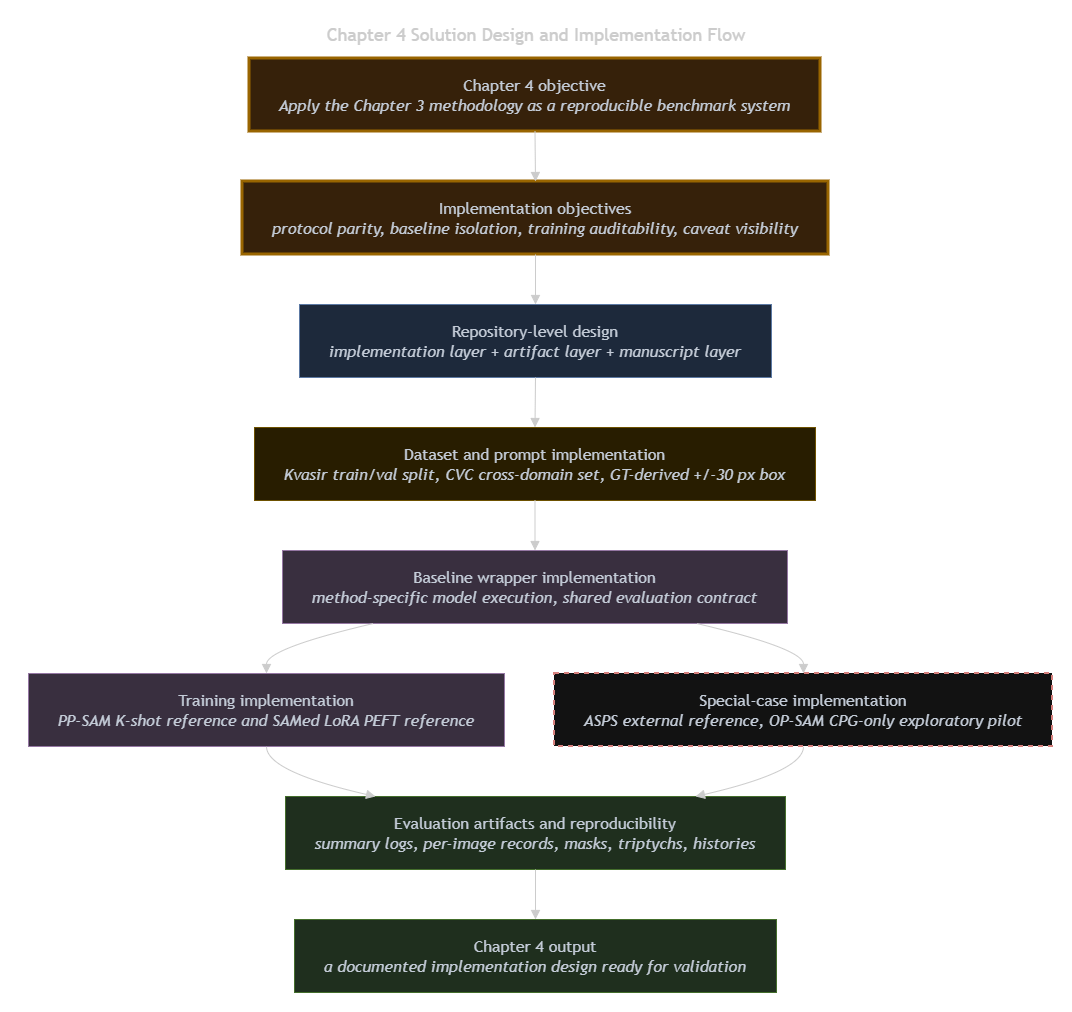
\includegraphics[width=0.88\textwidth]{figures/chapter4/fig_ch4_solution_implementation_flow.png}
\caption{Chapter~\ref{chap:solution} solution design and implementation flow. The figure summarises how the Chapter~\ref{chap:outline} methodology is applied as a reproducible benchmark system without extending into the Chapter~\ref{chap:validation} validation results.}
\label{fig:ch4-solution-flow}
\end{figure}


\section{Implementation Objectives}
\label{sec:impl-objectives}

The implementation operationalises the five research questions of Chapter~\ref{chap:intro}. RQ1 and RQ2 require a stable zero-shot evaluation pipeline for foundation-model scaling and medical pre-training transfer. RQ3 and RQ4 require training and checkpoint-management procedures for PP-SAM and SAMed LoRA. RQ5 requires special-case handling for prompt-free, fully supervised, and robustness-oriented extensions. Table~\ref{tab:implementation-objectives} summarises these objectives.

\begin{table}[H]
\centering
\caption{Implementation objectives and their relationship to the research questions.}
\label{tab:implementation-objectives}
\begin{tabular}{p{3.2cm}p{7.0cm}p{3.0cm}}
\toprule
\textbf{Objective} & \textbf{Implementation decision} & \textbf{RQ link} \\
\midrule
Protocol parity & Use the same held-out Kvasir split, CVC split, $\pm30$ box prompt, and metric definitions for v3-aligned baselines. & RQ1--RQ4 \\
Baseline isolation & Keep model-specific loading separate from the shared evaluation contract. & RQ1--RQ3 \\
Training auditability & Save checkpoints, histories, validation traces, summary files, and per-image records for training-based methods. & RQ3--RQ4 \\
Caveat visibility & Isolate ASPS and OP-SAM because their supervision or prompt assumptions differ from v3-aligned baselines. & RQ4--RQ5 \\
Future extensibility & Preserve per-image outputs so prompt-quality, scale, and boundary analyses can be added later. & RQ5 \\
\bottomrule
\end{tabular}
\end{table}

These objectives are deliberately conservative. The solution does not attempt to merge all models into a single universal inference function, because doing so would obscure method-specific assumptions. Instead, the implementation makes the shared parts explicit and documents every exception.

\section{Repository-Level Design}
\label{sec:repo-design}

The benchmark is organised into three functional layers. The implementation layer contains baseline-specific wrappers. The artifact layer stores summaries, per-image records, predictions, visualisations, training histories, and checkpoints. The manuscript layer consumes the consolidated artifact summaries and turns them into tables, figures, and discussion. The purpose of this design is traceability: a claim in the thesis should be traceable back to an authoritative result log and, where needed, to per-image records.

\begin{table}[H]
\centering
\caption{Repository-level design of the benchmark solution.}
\label{tab:repo-implementation-areas}
\begin{tabular}{p{3.1cm}p{5.0cm}p{5.2cm}}
\toprule
\textbf{Layer} & \textbf{Main artifacts} & \textbf{Design rationale} \\
\midrule
Implementation layer & SAM-family baseline wrappers and training scripts & Preserves method-specific model interfaces while enforcing a shared evaluation contract. \\
Artifact layer & Summary logs, per-image records, masks, triptychs, histories, and checkpoints & Makes aggregate results traceable and supports later failure analysis. \\
Manuscript layer & Chapter text, tables, figures, and bibliography & Reports only consolidated, verified results rather than copying transient intermediate outputs. \\
\bottomrule
\end{tabular}
\end{table}

This layered organisation also reduces the risk of stale interpretation. The consolidated experimental summary is treated as the authoritative result log for manuscript numbers, while the raw artifacts remain available for verification. When a new baseline or training run is added, the intended workflow is to update the artifacts first, then the consolidated result log, and only then the manuscript.

\section{Dataset and Prompt Implementation}
\label{sec:dataset-prompt-implementation}

The dataset implementation follows the split assumptions defined in Chapter~\ref{chap:outline}. Kvasir-SEG provides both the few-shot support pool and the held-out in-domain evaluation set. The 880-image training split is used for support sampling and fine-tuning, while the 120-image validation split is reserved for reporting in-domain performance. CVC-ClinicDB is used as a cross-domain evaluation set. This prevents the few-shot support examples from leaking into the reported Kvasir results and allows cross-dataset generalisation to be measured under the same metric suite.

The prompt implementation is designed as a controlled segmentation benchmark rather than as a full detection pipeline. For v3-aligned promptable baselines, the tight ground-truth box is expanded by 30 pixels in each direction and used as the inference prompt. This fixed prompt setting has two advantages. First, it avoids giving one method a cleaner prompt than another. Second, it makes prompt quality a controlled variable: the current stage fixes one perturbation level, while the next stage can extend the same implementation to multiple perturbation levels such as 0, 10, 30, and 50 pixels.

ASPS and OP-SAM do not use this prompt implementation in the same way. ASPS is a dense fully supervised model and therefore has no v3 box prompt at inference time. OP-SAM generates its own prompt from a support image rather than consuming the ground-truth-derived v3 box. These differences are not treated as implementation bugs; they are documented as protocol differences and interpreted separately.

\section{Baseline Wrapper Implementation}
\label{sec:baseline-wrapper-implementation}

The baseline wrappers translate heterogeneous model interfaces into a common evaluation flow. Each wrapper discovers image--mask pairs, loads the required checkpoint, prepares the method-specific input representation, runs inference, converts the output mask back to the original image resolution when necessary, computes the metric suite, and writes the standard artifacts. This flow is shared at the design level even though the internal model calls differ across families.

\begin{table}[H]
\centering
\caption{Baseline wrapper families and their role in the solution design.}
\label{tab:baseline-wrapper-roles}
\begin{tabular}{p{3.4cm}p{3.8cm}p{6.0cm}}
\toprule
\textbf{Family} & \textbf{Examples} & \textbf{Implementation role} \\
\midrule
Zero-shot foundation models & SAM ViT-B/L/H, SAM2 Hiera-S/B+/L & Evaluate backbone scaling while keeping the prompt and metric contract fixed. \\
Medical-transfer baseline & MedSAM & Test whether generic medical pre-training transfers to endoscopic polyp data. \\
Few-shot adaptation & PP-SAM 1/5/10-shot & Implement the full-encoder prompt-perturbation reference. \\
Parameter-efficient adaptation & SAMed LoRA 1/5/10-shot and full 880 & Implement the Adapter/LoRA PEFT extension required by the project brief. \\
Special entries & ASPS, OP-SAM & Preserve external and exploratory evidence without forcing incompatible protocols into one ranking. \\
\bottomrule
\end{tabular}
\end{table}

This wrapper design is important for fairness. If all methods were forced through exactly the same internal function call, method-specific assumptions such as SAM2 predictor state, LoRA checkpoint loading, or OP-SAM support conditioning could be broken. If every wrapper used its own metric and artifact code, the comparison would become difficult to audit. The adopted design is a compromise: method-specific execution is allowed, but evaluation outputs must follow the shared contract.

\section{Few-Shot and LoRA Training Implementation}
\label{sec:training-implementation}

The current-stage benchmark contains two training-based adaptation recipes. PP-SAM represents full-encoder prompt-perturbation fine-tuning under a small support budget. For each support size, the support images are sampled from the Kvasir training split, and the selected checkpoint is evaluated on the held-out Kvasir validation split and CVC-ClinicDB. SAMed LoRA represents parameter-efficient adaptation. It injects rank-4 low-rank updates into SAM ViT-B attention projections and trains a smaller set of parameters together with the prompt and mask decoding components.

The training implementation records validation histories instead of relying only on the final training epoch. This design choice matters because low-shot training can overfit rapidly. A model may continue to reduce training loss while its validation Dice decreases. Saving histories and best-checkpoint metadata therefore makes the training decision auditable and supports later interpretation in Chapter~\ref{chap:validation}.

The full-training SAMed run is included for a different reason from the K-shot runs. The K-shot runs test whether LoRA can match prompt-perturbation fine-tuning under the same limited support budget. The full 880-sample run tests whether the LoRA capacity is sufficient when the training signal is no longer extremely small. This distinction is why SAMed appears in both RQ3 and RQ4.

\section{Special-Case Implementations}
\label{sec:special-case-implementation}

Two implemented entries intentionally remain outside the main v3 ranking. ASPS is handled as a fully supervised external upper-bound reference. The available checkpoint follows the PraNet training protocol, whose training set overlaps with the standard Kvasir and CVC data used elsewhere in the project. Evaluating this checkpoint on the v3 Kvasir/CVC split would invalidate the implementation-level comparison by mixing training and test images. The solution is to evaluate the released checkpoint only on the PraNet held-out test subset and to reserve a v3-aligned ASPS retraining for future work.

OP-SAM is handled as an exploratory prompt-free pilot. Its current implementation uses the Cascaded Prior Generator path and a support image, but it does not include the full CPG+SPF+EPE pipeline of the original paper. The implementation is still useful because it tests whether support-conditioned, training-free prompt generation can provide a competitive alternative to prompt-end fine-tuning. However, the result is interpreted as evidence about the current CPG-only implementation, not as a final judgement on full OP-SAM.

\section{Evaluation Artifacts and Reproducibility}
\label{sec:artifact-reproducibility}

The output schema is part of the solution design. A benchmark is reproducible only if the reported aggregate numbers can be traced back to the evaluation artifacts that produced them. For this reason, each evaluation writes a dataset-level summary and a per-image record. The summary stores aggregate metrics and model metadata. The per-image record stores image identifiers, metric values, and runtime information. When supported, predicted masks and visual triptychs are also saved for qualitative inspection.

\begin{table}[H]
\centering
\caption{Evaluation artifacts used to support reproducibility and peer review.}
\label{tab:evaluation-artifacts-ch4}
\begin{tabular}{p{3.4cm}p{6.2cm}p{4.0cm}}
\toprule
\textbf{Artifact type} & \textbf{Content} & \textbf{Use in thesis} \\
\midrule
Dataset summary & Mean and standard deviation for Dice, IoU, precision, recall, HD95, FPS, and metadata & Populates the quantitative tables in Chapter~\ref{chap:validation}. \\
Per-image records & Image-level metrics, image identifiers, and runtime information & Supports failure analysis and future object-scale stratification. \\
Predicted masks & Binary output masks saved where supported & Enables visual inspection and downstream re-analysis. \\
Triptych figures & Image, ground-truth mask, and prediction panels & Supports qualitative analysis in Chapter~\ref{chap:validation}. \\
Training histories & Epoch-level validation traces and best-checkpoint metadata & Justifies checkpoint selection and overfitting discussion. \\
\bottomrule
\end{tabular}
\end{table}

The consolidated experimental summary is used as the authoritative result log for manuscript numbers. This avoids copying partially updated results from older experiments and reduces the risk that Chapter~\ref{chap:validation} contradicts the artifacts. The chapter therefore closes the design-and-implementation part of the thesis: the system has defined a protocol, implemented method-specific wrappers under that protocol, separated non-aligned entries, and preserved artifacts for review. The next chapter validates the implemented benchmark through quantitative and qualitative results.
